\documentclass{article}[18pt]
\usepackage{../../../../../format}
\lhead{CSys - Operating Systems}


\begin{document}
\begin{center}
\underline{\huge Introduction to Operating Systems}
\end{center}
\subsection{Definition}
A program that acts as an intermediary between a user and the hardware
\subsection{Goals}
\begin{itemize}
	\item Execute user programs
	\item Make solving user programs easier
	\item Make the computer system convenient to use
	\item Use the resources of the systems fairly and efficiently
\end{itemize}
\subsection{Components}
An operating system is a:
\begin{itemize}
	\item \textbf{Resource allocator}: Responsible for the management of the computer system resources
	\item \textbf{Control Program}: Controls the execution of user programs and operation of the I/O devices
	\item \textbf{Kernel}: The one program that runs all the time
\end{itemize}
A process is a unit of execution; an abstraction that is used to support the discussion and study of operating systems\\
Resources needed by the process include: CPU time, memory, files and I/O devices\\
The resources may be allocated at the start of a process or as it executes\\
Executes (performs its work) using its associated resources; a collection of instructions that carry out a reasonable task.\\
\\
The operating system is responsible for process management including:
\begin{itemize}
	\item Process creation and deletion
	\item Process holding and resuming
	\item Mechanisms for process synchronization
\end{itemize}
\section{The process concept}
A process includes:
\begin{itemize}
	\item Code: text section
	\item Current activity, represented by the program counter and the content of the CPU's registers
	\item Data stack: Temporary data such as local variables
	\item Data section: Global variables
	\item Heap: Memory allocated while the process is running
\end{itemize}
\section{Process Control Block}
Information about each process is represented by a process control block (PCB) including
\begin{itemize}
	\item Unique identifier
	\item State
	\item CPU Utilisation
	\item CPU scheduling information
	\item Memory usage
	\item Other information
\end{itemize}
\section{Process state}
As a process executes, it changes state:
\begin{itemize}
	\item New - The process is being created
	\item Running - instructions are being executed
	\item Waiting - The process is waiting for some event to occur
	\item Ready - The process is ready to be dispatched to the CPU
	\item Terminated - The process has completed its execution, or some other event causing termination
\end{itemize}
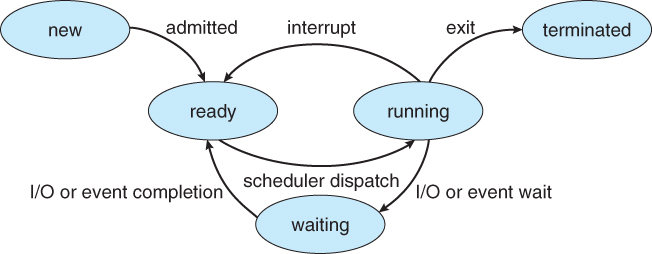
\includegraphics[scale=0.7]{state.jpg}
\section{Process Creation}
A new process, as a parent processes, can create a number of child processes, which, in turn create other processes, forming a tree of processes.\\
\\
Resource sharing: three possible cases:
\begin{itemize}
	\item The parent and child processes share all resources
	\item The child process shares a subset of the parent's resources
	\item The parent and child process share no resources
\end{itemize}
Execution: two possible cases:
\begin{itemize}
	\item The parent and child execute concurrently
	\item The parent waits until the child terminates
\end{itemize}
\section{Process Termination}
The process executes its last statement and asks the operating system to delete it:
\begin{itemize}
	\item Outputs the data from the child's process to parent
	\item The child process's resources are de-allocated by operating system
\end{itemize}
The parent process may terminate execution of the child processes if:
\begin{itemize}
	\item The child process has exceeded its allocated resources
	\item The task assigned to child is no longer required
	\item The parent itself is terminating (cascade termination)
\end{itemize}
\section{The Kernel}
\textbf{Aim:} To provide an environment in which processes can exist\\
\\
Four essential components:
\begin{itemize}
	\item Privileged instruction set
	\item Interrupt mechanism
	\item Memory protection
	\item Real time clock
\end{itemize}
The kernel consists of:
\begin{itemize}
	\item The first-level interrupt handler: to manage interrupts
	\item The dispatcher: to switch the CPU between processes
	\item Intra operating system communications
\end{itemize}
\section{Interrupts}
\subsection{Definition}
An interrupt is a signal from either hardware or software of an event that will cause a change of process, for example:
\begin{itemize}
	\item \textbf{Hardware}: Triggers an interrupt by sending a signal to the CPU via the system bus e.g. I/O event
	\item \textbf{Software}: Triggers an interrupt by sending a system call for some action by the operating system
\end{itemize}
\textbf{Interrupt Routines}: OS routines that execute whenever an interrupt occurs
\section{First level interrupt handler}
The function of the FLIH is to:
\begin{itemize}
	\item Determine the source of the interrupt (prioritise)
	\item Initiate servicing of the interrupt (selection of suitable process of the dispatcher)
\end{itemize}
\section{Privileged instructions}
Some instructions must be accessible only to the operating system: \textbf{privileged instruction set}.\\
\\
Privileged instructions include functions such as:
\begin{itemize}
	\item Managing interrupts 
	\item Performing I/O
	\item Halting a process
\end{itemize}
\section{Dual mode}
\textbf{Aim}: To distinguish between execution of operating system code and user defined code. We do not let the user execute instructions that could cause harm.\\
\\
Two modes:
\begin{itemize}
	\item User mode
	\item Kernel mode
\end{itemize}
\section{Privileged Instructions}
Switching from user mode to kernel mode occurs when:
\begin{itemize}
	\item A user process calls on the operating system to execute a function needing a privileged instruction
	\item An interrupt occurs
	\item An error condition occurs in the user process
	\item An attempt is made to execute a privileged instruction while in user mode
\end{itemize}
\section{The dispatcher}
\begin{itemize}
	\item Assigns processing resources for processes
	\item Is later initiated when
	\begin{itemize}
		\item A current process cannot continue
		\item The CPU may be better used elsewhere, for instance:
		\begin{itemize}
			\item After an interrupt changes a process state
			\item After a system call which results in the current process not being able to continue
			\item After an error which causes a process to suspend
		\end{itemize}
	\end{itemize}
\end{itemize}
\end{document}